\documentclass[../../thesis.tex]{subfiles}
\graphicspath{{\subfix{diagrams/}}}

% \begin{document}
This section will present the results of the proposed implementation, introducing several metrics that quantify the system's capabilities and limitations. In zkSNARK enabled systems, the results must always be considered out of two different points of view. For one, gas savings are essential. After all, this system is built to reduce gas consumption per trade. Another thing to consider is the performance of the zkSNARK steps necessary to execute and verify an aggregation batch. As zkSNARKs rely on complex cryptographic primitives, the generation of proofs is computationally demanding, resulting in demanding hardware requirements and long execution times. As this system's primary goal is to reduce the required gas per trade on Uniswap, we will begin with these results. After, we will look at the performance results of the zkSNARK circuits, which gives a good understanding of the current limitations of the technology.

\subsection{Gas Cost}
In this system, we have four different operations that require gas to be executed. We will now look at these operations, presenting the measured results. The following three charts are scaled logarithmically on the x-axis. The logarithmical scale was chosen, as these operations have a significant overhead (fixed cost) and a proportionally small amount of variable cost. The way fixed and variable costs are distributed results in the cost per trade to reduce significantly initially, which can be visualized best on a logarithmic x-axis scale.

\subsubsection{Trade Aggragation}
To break down the gas cost of a trade aggregation batch, we must first differentiate between the fixed and variable gas costs that need to be paid per batch and trade. For one, the gas for the net-trade, executed on Uniswap, must be paid. The gas required for executing the net-trade varies, depending on the direction of the net-trade, ~142k when trading from Ether and ~167k gas when trading from an ERC20 token.
 
Another fixed cost to consider is the gas for verifying the zkSNARK proof, handling the refund payment of the aggregator and the on-chain checks, costing ~342k gas per aggregation batch. The combined fixed amount of gas per aggregation batch is 484k/509k gas, depending on the net-trades direction. For each trade in a batch, we must pay 6619 gas, which is used for recreating the data hash and emitting the BalanceUpdate event. When using these numbers, we get the following cost per trade, depending on the batch size. This diagram uses the more expensive net-trade (ERC20 to Ether) to calculate the results, which is the upper bound cost per trade for the corresponding batch size. As the difference is small, the difference in gas per trade converges quickly. The theoretical maximum batch size is 1811, which is where Ethereums block gas limit is reached. 

To compare the results of an unaggregated Uniswap trade, we define a break-even price equal to the cost of a Uniswap trade. Our system makes economic sense once our gas per trade cost is lower than the break-even point. We will use 142k gas as our break-even point, which is the best case for a Uniswap trade. Theses results, presented in F. \ref{fig:cost_trade}, do not contain any gas cost required for making a deposit or withdrawal.

\begin{figure}[h]
    \centerline{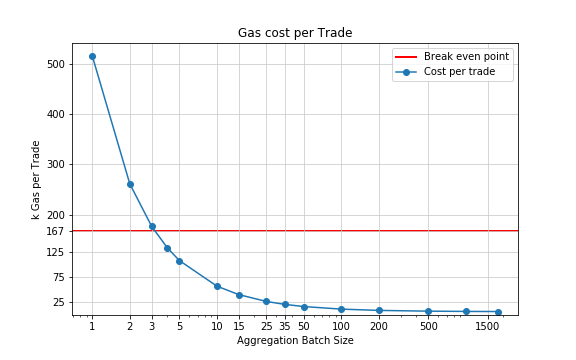
\includegraphics[totalheight=6cm]{diagrams/trade_cost.png}}
    \caption{Gas cost: per trade and breakeven point}
    \label{fig:cost_trade}
\end{figure}

\subsubsection{Deposits and Withdrawals}
Before a user can trade, funds must be deposited into the system. Presenting these results is a bit more complex compared to the trade aggregation results for two reasons. For one, the deposits and withdrawals are aggregated as one aggregation batch. Since the gas costs for a deposit and withdrawal are different, and the number of deposits and withdraws included in a batch is not predictable, the cost per deposit/withdrawal depends on the proportion of these operations. On top of that, the gas cost of a deposit/withdrawal also depends on the asset. Ether deposits/withdrawals are cheaper than ERC20, which is a result of how tokens are represented on the Ethereum blockchain. Thus, we will present three quartiles for deposits and withdraws, representing the share of an asset in the batch. For example, as seen in F. \ref{fig:cost_dep}, `25\% Eth' represents the gas cost per deposit if 25\% of deposits in that batch are Ether deposits. While the numbers are a bit inaccurate for smaller batch sizes, it seems like the best approach to present the results overall. 

\paragraph{Deposit Aggregation:}
As with the trade aggregation, there is a fixed and variable gas cost required per batch. For each deposit aggregation, results presented in F. \ref{fig:cost_dep}, we have ~312k gas as a fixed cost. This amount covers all checks and verifications explained in S. \ref{aggr_deps}. The variable gas cost depends on the type of asset being deposited. Depositing an ERC20 token requires significantly more gas than depositing Ether, as multiple smart-contract interactions are necessary. An Ether deposit adds ~44k gas, an ERC20 deposit ~128k gas. The maximum batch size is calculated by checking how many deposits can fix in a block if only the most expensive operation is included. In our case, a batch only containing ERC20 deposits is the most expensive scenario, resulting in a maximum batch size of 94.

\begin{figure}[h]
    \centerline{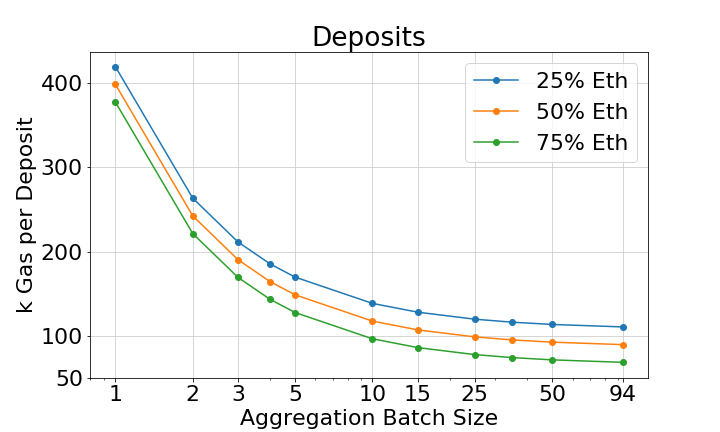
\includegraphics[totalheight=6cm]{diagrams/dep_ET_.png}}
    \caption{Gas cost: per deposit assuming different share of Ether deposits}
    \label{fig:cost_dep}
\end{figure}

\paragraph{Withdrawal Aggregation:}
The fixed costs of the withdrawals is equal to the amount specified in the deposit aggregation, as they are being verified in the same batch. As with the deposits, the variable withdrawal cost is different, depending if Ether or an ERC20 token is withdrawn. An Ether withdrawal adds ~19k gas, an ERC20 withdrawal ~65k gas. The maximum batch size is chosen based on the worst-case propotions, in this case only ERC20 withdraws and the number of deposits we can include before Ethereum block gas limit is reached. For withdrawals, results presented in F. \ref{fig:cost_with}, thats a maximum batch size of 186.

\begin{figure}[h]
    \centerline{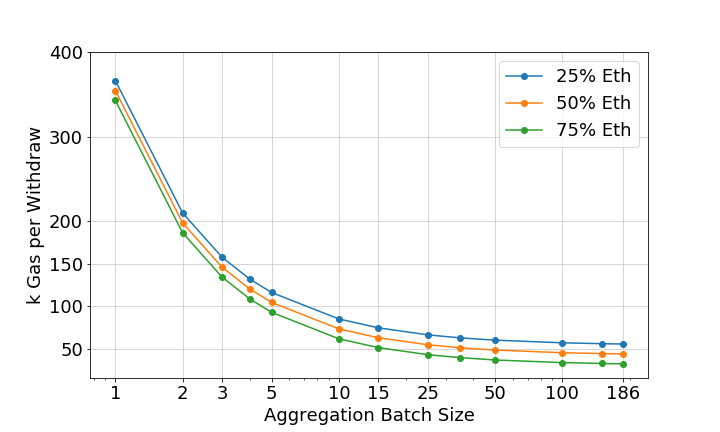
\includegraphics[totalheight=6cm]{diagrams/with_ET_.png}}
    \caption{Gas cost: per withdraws assuming different share of Ether withdrawals}
    \label{fig:cost_with}
\end{figure}

\paragraph{Combining Deposit and Withdrawal Gas Cost:}
Modeling the combined gas costs of deposits and withdraws is omitted in this work, as many assumptions are required to calculate this. As mentioned before, the proportion of Ether and ERC20 operations and the proportion of deposits and withdrawals influence the results. For the deposits and withdrawals, a valid approach was taken to model the potential gas cost, depending on the proportional share of funds. Combining these values, defining the proportional share of deposits and withdrawals in an aggregation batch would not yield representative results, as several valid combinations would need to be considered. The diagrams presented above give a clear indication of the potential cost, which suffices for this work.  

\paragraph{Instant Withdrawals:}
The cost of instant withdraws is also worth considering. Since we are not batching instant withdraws, there is only a fixed cost per withdrawal that needs to be paid. Since instant withdrawals are not implemented at the time of writing, a rough estimate of the gas costs can only be provided. To update a balance in a Merkle tree with a depth of 16, we need to hash a total of 34 times. 32 times for the Merkle inclusion proof and update, twice for hashing the old and new balance. Computing a MiMC hash currently costs ~38k gas, bringing the cost to around ~1.3m gas per instant withdrawal.

\subsection{zkSNARK Circuit Metrics}
Another aspect to consider is the performance of the zkSNARK circuits. The benchmarks for the zkSNARK circuits where performed on a Google Cloud Plattform C2 instance, with 60 vCores (3.1GHz base and 3.8GHz turbo clock speed) and 240Gb of memory. This instance was chosen because of the large amount of memory and the fast clock speed. The number of cores does not impact the benchmarking results, as the zkSNARK steps cannot be parallelized at the time of writing.

\subsubsection{Execution Time}
The first obvious metric to consider is the execution time of the different steps required when using zkSNARK circuits. As we will see in the following sections, using zkSNARK circuits requires powerful hardware. We will begin by looking at the performance metrics based on execution times first and then look at more hardware-specific metrics. 

\paragraph{Compilation and Setup:}
Before we can generate any zkSNARK proofs, we have to compile our circuits and run the setup. These two steps only need to be run once per circuit, so they are not significant for the viability of this system. However, the results, presented in F. \ref{fig:comp_setup_time}, were measured during the benchmarking, so it would feel incomplete not to present them. 

\begin{figure}[h]%
    \centering
    \subfloat[]{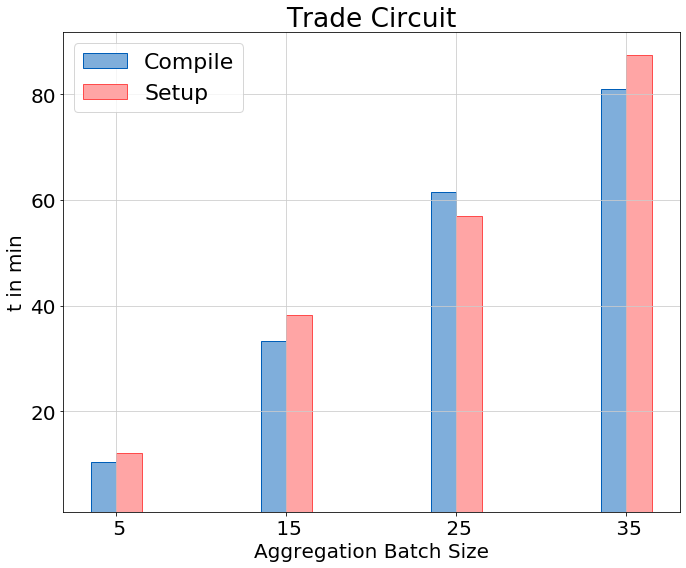
\includegraphics[width=5.9225cm]{diagrams/results_final_trade-compile-setup-time.png} }%
    \qquad
    \subfloat[]{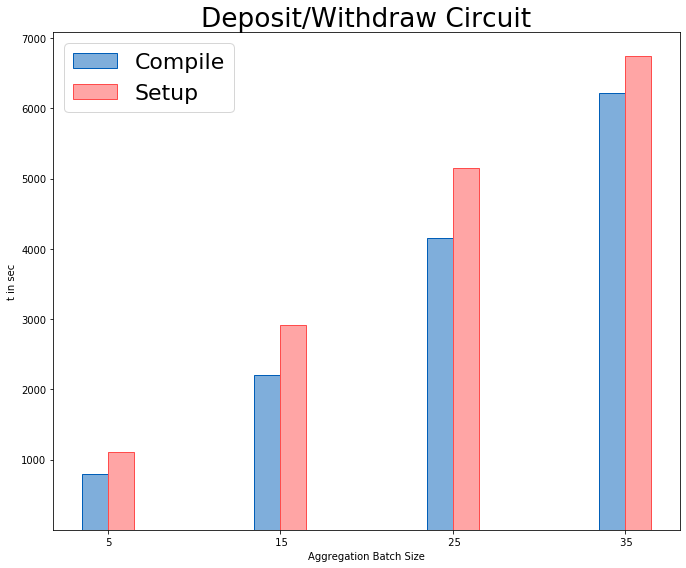
\includegraphics[width=5.9225cm]{diagrams/results_final_dep-compile-setup-time.png} }%
    \caption{Execution time: Compilation and setup}%
    \label{fig:comp_setup_time}%
\end{figure}

\paragraph{Witness Computations and Proof Generation:}
For each aggregation batch, we need to run the witness computation first.  After the witness computation is complete, the proof can be generated. As these two steps are required for every aggregation batch, the execution, presented in F. \ref{fig:witness_proof_time}, times impact the practical viability of the system. 

\begin{figure}[h]%
    \centering
    \subfloat[]{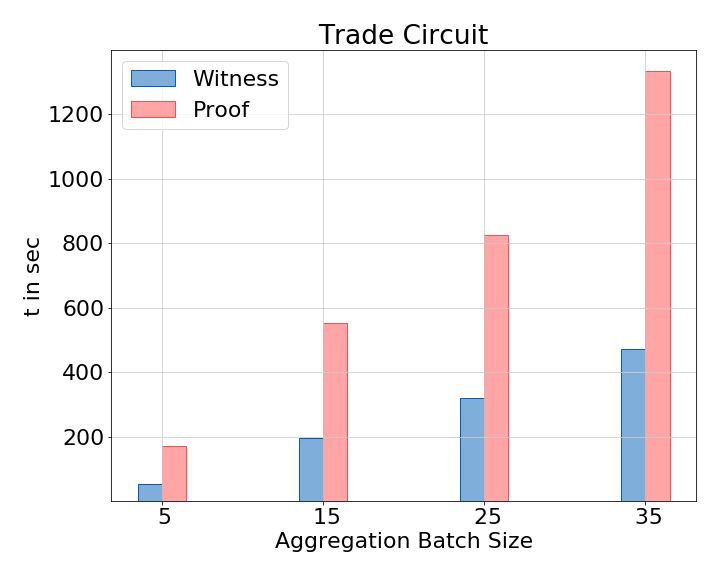
\includegraphics[width=5.9225cm]{diagrams/results_final_trade-witness-proof-time.png} }%
    \qquad
    \subfloat[]{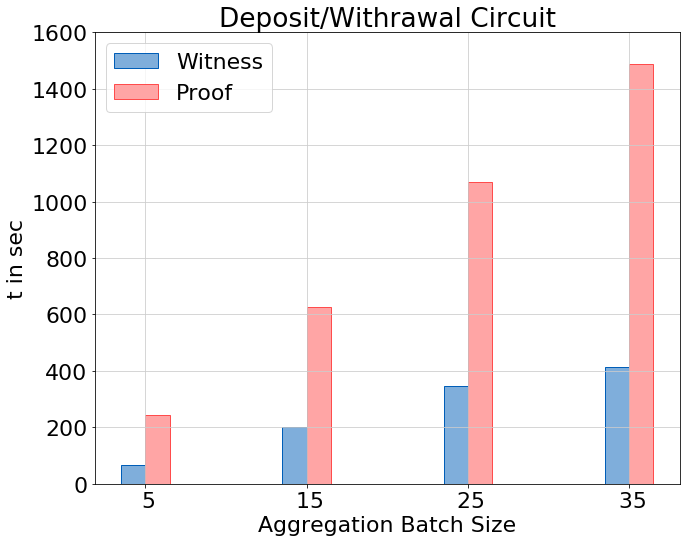
\includegraphics[width=5.9225cm]{diagrams/results_final_dep-witness-proof-time.png} }%
    \caption{Execution time: Witness computation and proof generation}%
    \label{fig:witness_proof_time}%
\end{figure}

\subsubsection{Memory Usage}
Only looking at the execution times gives us an idea of how many operations can be batched. It tells us nothing about the hardware requirements needed for working with circuits of this size. One thing to look at is the memory used in the different steps. In general, the memory consumption of these processes is high, which is why a server instance with such a large amount of memory was chosen. 

\paragraph{Compilation and Setup:}
When measuring the compilation memory consumption, presented in F. \ref{fig:comp_setup_mem}, we get a confusing picture. The results do not really make sense, as smaller circuits sometimes require more memory than smaller ones. However, the measurements were repeated on different machines and operating systems, always resulting in inconclusive results. The memory measurement script uses the command line tool `ps' to take these measurements, which measures reserved memory by a process. Alternatively, a profiler could be used to measure the actual memory usage. Using a profiler would severely impact the application's performance, which is why it was not attempted. As these steps only have to be executed once, they are not a meaningful metric. 

\begin{figure}[h]%
    \centering
    \subfloat[]{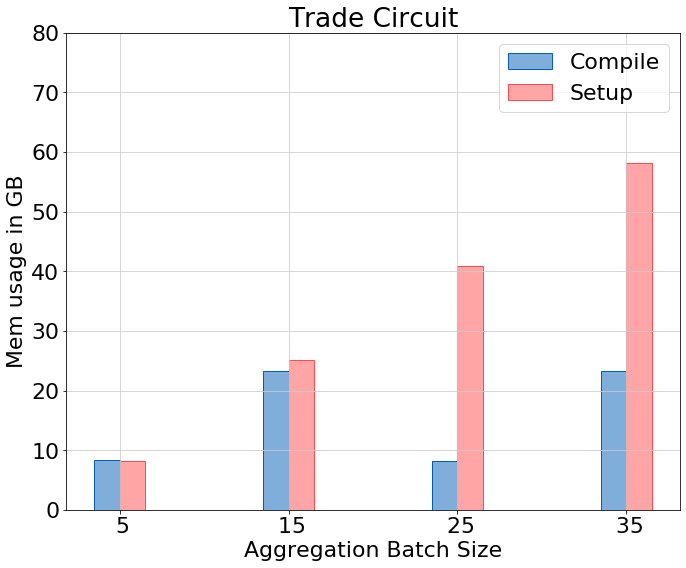
\includegraphics[width=5.9225cm]{diagrams/results_final_trade-compile-setup-mem.png} }%
    \qquad
    \subfloat[]{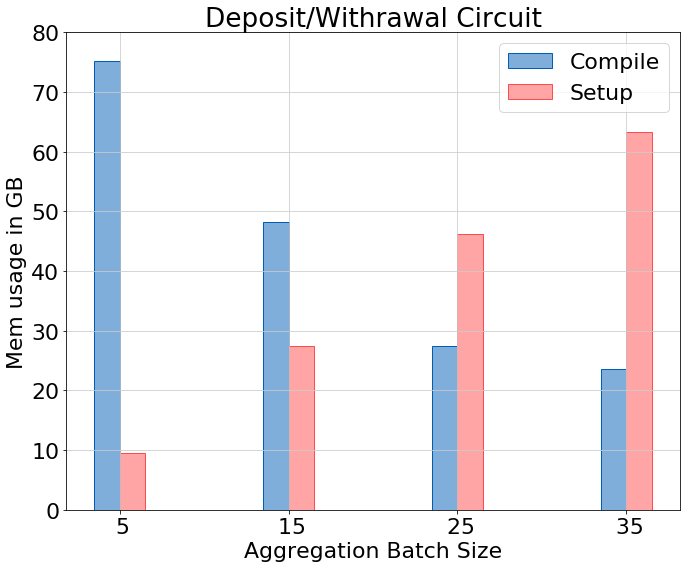
\includegraphics[width=5.9225cm]{diagrams/results_final_dep-compile-setup-mem.png} }%
    \caption{Memory consumption: compilation and setup }%
    \label{fig:comp_setup_mem}%
\end{figure}

\paragraph{Witness Computation and Proof Generation:}
The memory required for running the witness computation and proof generation, presented in F. \ref{fig:witness_proof_mem}, is an important metric and dictates the hardware requirements for the aggregation process. We need to run these steps for every aggregation batch, so hardware capable of handling the memory requirements must be available.

\begin{figure}[h]%
    \centering
    \subfloat[]{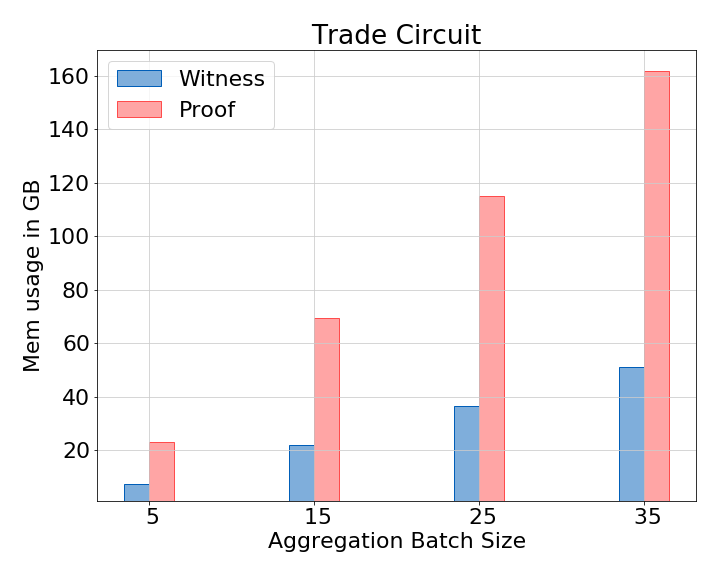
\includegraphics[width=5.9225cm]{diagrams/results_final_trade-witness-proof-mem.png} }%
    \qquad
    \subfloat[]{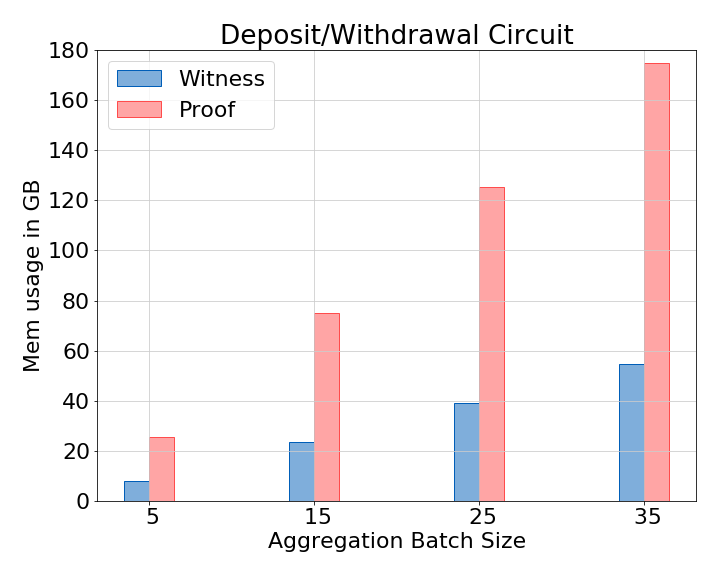
\includegraphics[width=5.9225cm]{diagrams/results_final_dep-witness-proof-mem.png} }%
    \caption{Memory consumption: witness computation and proof generation}%
    \label{fig:witness_proof_mem}%
\end{figure}

\subsubsection{Constraints}
Looking at the results in F. \ref{fig:constraints}, we see that the execution times increase linearly with the batch size. The same pretty much goes for the memory consumption of our circuits. In general, the complexity of a zkSNARK circuit is defined by the number of constraints the circuit is made of. Each additional element in the batch adds a certain number of constraints to the circuit.  Looking at our circuits, we get the following constraint counts for different batch sizes. 

\begin{figure}[h]%
    \centering
    \subfloat[]{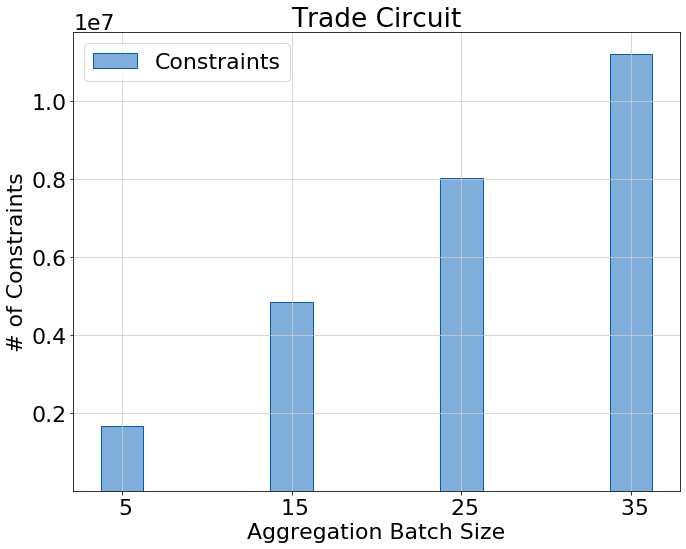
\includegraphics[width=5.9225cm]{diagrams/results_final_trade-constraints.png} }%
    \qquad
    \subfloat[]{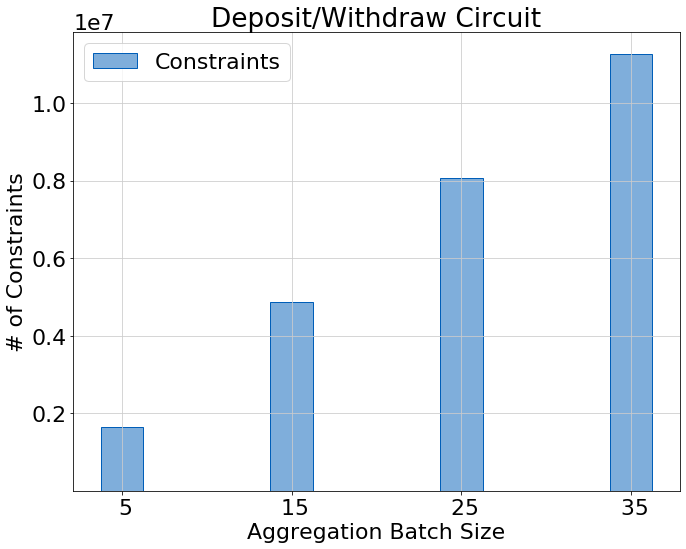
\includegraphics[width=5.9225cm]{diagrams/results_final_dep-constraints.png} }%
    \caption{Constraint count of circuits for different batch sizes}%
    \label{fig:constraints}%
\end{figure}

\paragraph{Origin of Constraints:}
Both circuits can be broken down into three different main segments that add a certain number of constraints. 1) We need to run the inclusion proof and update the Merkle tree. 2) We check the signature and if the balance update follows the signed amounts. 3) We need to compute the data hash. For each of these operations, we get constraint numbers that are added per additional batch element. These numbers were measured by compiling the segments separately and checking the constraint count. Comparing these to the total constraint values, we realize that they are higher than expected. The increased number of constraints can be explained by the ZoKrates optimizer, which runs several optimizations during compilation. As we can see, the final hash produces significantly more constraints, which is caused by creating the deposit and withdrawal hash.

\begin{table}[h]
    \centering
    \begin{tabular}{lll}
    \toprule
                                  & Fixed Cost: & Variable Cost:     \\ \hline
    \multicolumn{3}{l}{\textbf{Trade Circuit:}}                      \\ \hline
    \midrule
    Merkle Tree                   & 1          & 179781              \\ \hline
    Verify sig and balance update & 1175       & 25675               \\ \hline
    Data hash                     & 182254     & 184806              \\ \hline
    \multicolumn{3}{l}{\textbf{Deposit/withdrawal Circuit:}}           \\ \hline
    \midrule
    Merkle Tree                   & 1           & 179781              \\ \hline
    Verify sig and balance update & 1           & 28154               \\ \hline
    Data hash                     & 111172      & 395076              \\ \hline
    \bottomrule
    \end{tabular}
\end{table}  \label{constraint_source}

\paragraph{Hashing and Constraints:} \label{hashing_const}
The MiMC hashing algorithm was used for hashing the Merkle tree, as it is efficient to use in zkSNARK circuits. The most common hashing operation used in the system is the pair hashing of the Merkle tree. Every balance update requires 34 pair hashes, one for hashing the old balance, 16 for the Merkle inclusion proof, one for hashing the new balance, and 16 for updating the Merkle tree. We must also remember that the pair elements need to be sorted according to their position (left, right), which doubles the constraints in a zkSNARK circuit. On the other hand, we also need to hash the balances in the zkSwap smart-contract for recreating the data hash. In Solidity, the SHA256 hashing algorithm is a lot cheaper than MiMC. Since we have to recreate the data hash for every batch we want to verify on-chain, the data hash is computed with the SHA256 hashing algorithm. 

\begin{table}[h]
    \centering
    \begin{tabular}{lll}
    \toprule
    Hashing Op         & Constraints & Gas Usage \\  \hline
    \midrule
    MiMC pair          & 2642        & 38840    \\  \hline
    MiMC pair sorted   & 5285        & 38840    \\  \hline
    SHA256 pair        & 56227       & 2179     \\  \hline
    SHA256 pair sorted & 112453      & 2179     \\  \hline
    \bottomrule
    \end{tabular}
\end{table}

\paragraph{Constraints Processed per Second:}
The last metric we want to introduce is constraints processed per second in the witness computation and proof generation step. We can calculate these values by dividing the execution time by the number of constraints. At the time of writing, these steps are not parallelizable and only run on one CPU core. The Loopring protocol claims to have parallelized the libsnark library\footnote{https://github.com/scipr-lab/libsnark}, which we will look at in S. \ref{para_loopring}. For this reason, we are introducing this metric, as we can compare the outcomes and the potential speedup of parallelizing. This metric can also be helpful to test the performance of the circuits on a CPU with a higher clock speed.

\begin{table}[]
    \centering
    \begin{tabular}{lll}
    \toprule
    Batch Size & Witness: constraints / sec & Proof: constraints / sec \\
    \midrule
    5           & 27604                     & 9685                    \\
    15          & 29615                     & 8417                    \\
    25          & 29088                     & 9612                    \\
    35          & 27797                     & 8382                    \\
    \midrule
    Average     & 28526                     & 9024                    \\
    \bottomrule 
    \end{tabular}
\end{table}\label{const_per_sec}

